\documentclass[svgnames,11pt]{beamer}
\input{/home/tof/Documents/Cozy/latex-include/preambule_commun.tex}
\input{/home/tof/Documents/Cozy/latex-include/preambule_beamer.tex}
%\usepackage{pgfpages} \setbeameroption{show notes on second screen=left}
\author[]{Christophe Viroulaud}
\title{Encodage des caractères}
\date{\framebox{\textbf{DonRep 14}}}
%\logo{}
\institute{Première - NSI}

\begin{document}
\begin{frame}
\titlepage
\end{frame}
\begin{frame}
    \frametitle{}

    En première approche il semble simple de représenter une chaîne de caractère en mémoire : il
suffit d’associer un numéro (un code binaire) à chaque lettre.
\begin{center}
    \begin{tabular}{|*{5}{c|}}
        \hline
        01100001&01100010&01100011&01100100&01100101\\
        \hline
        97&98&99&100&101\\
        \hline
        a&b&c&d&e\\
        \hline
    \end{tabular}
\end{center}
\end{frame}
\begin{frame}
    \frametitle{}

    En pratique plusieurs contraintes apparaissent. Il faut par exemple que chaque système respecte le même encodage. De plus tous les caractères doivent être représentés.
\begin{multicols}{2}
    \begin{center}
        \begin{tabular}{|*{5}{c|}}
            \hline
            97&98&99&100&101\\
            \hline
            a&b&c&d&e\\
            \hline
        \end{tabular}
        \captionof{table}{machine 1}
    \end{center}
    \begin{center}
        \begin{tabular}{|*{5}{c|}}
            \hline
            97&98&99&100&101\\
            \hline
            !&@&:&\#&é\\
            \hline
        \end{tabular}
        \captionof{table}{machine 2}
    \end{center}
\end{multicols}
\begin{center}
    {\Large Héloïse $\Rightarrow$ H@elo\&ése} 
\end{center}
\end{frame}
\begin{frame}
    \frametitle{}

    \begin{framed}
        \centering Comment encoder les caractères en mémoire?
    \end{framed}

\end{frame}
\section{Première tentative de normalisation: ASCII}
\begin{frame}
    \frametitle{Première tentative de normalisation: ASCII}

    \begin{itemize}
        \item <1-> Années 50, lors de l’apparition des premiers ordinateurs, chaque matériel utilisait son propre système de codage.
        \item <2-> Début des années 60, l'ANSI (American National Standards Institute) propose une première tentative de normalisation : \textbf{l’ASCII}.
    \end{itemize}

\end{frame}
\begin{frame}
    \frametitle{}

   \begin{aretenir}[]
    \begin{itemize}
        \item ASCII: American Standard Code for Information Interchange (Code américain normalisé pour l'échange d'information)
        \item Un caractère est encodé sur 7 bits. En pratique 1 octet est utilisé; le bit de poids fort (bit de gauche) sert de somme de contrôle.
    \end{itemize}
   \end{aretenir}

\end{frame}
\begin{frame}
    \frametitle{}

    \begin{activite}
    \begin{enumerate}
        \item Combien de caractères peut-on représenter en ASCII?
        \item La lettre \textbf{A} est représenté par le code binaire: \texttt{\textbf{01000001}}. Calculer la valeur décimale représentant la lettre A.
        \item Calculer la valeur hexadécimale représentant la lettre A.
    \end{enumerate}
    \end{activite}

\end{frame}
\begin{frame}
    \frametitle{Correction}


        {\Large $$2^7=128$$}


\end{frame}
\begin{frame}
    \frametitle{}

    {\Large $$01000001$$}
    {\Large $$1×2^0+1×2^6=65$$}


\end{frame}
\begin{frame}
    \frametitle{}
{\Large
    \begin{center}
        \begin{tabular}{ccc}
            caractère&\multicolumn{2}{c}{a}\\ 
            binaire&0100&0001\\
            hexadécimal&4&1\\
        \end{tabular}
    \end{center}
}
\begin{center}
\centering
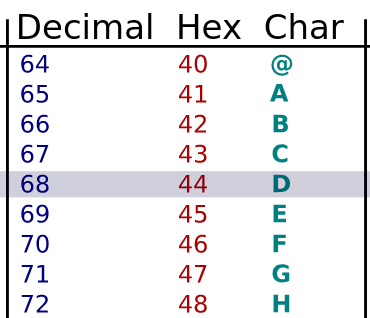
\includegraphics[width=6cm]{ressources/ascii.png}
\captionof{figure}{Extrait de la table ASCII}
\label{IMG}
\end{center}
\end{frame}
\begin{frame}
    \frametitle{}

    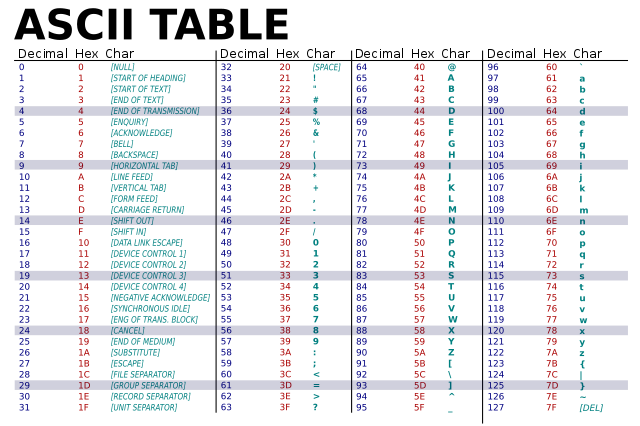
\includegraphics[width=10cm]{ressources/ascii-all.png}

\end{frame}
\begin{frame}
    \frametitle{}

    \begin{aretenir}[Remarque]
    La table ASCII ne permet pas de représenter les caractères accentués, les idéogrammes\dots
    \end{aretenir}

\end{frame}
\section{Prise en compte des différents langages: ISO 8859}
\begin{frame}
    \frametitle{Prise en compte des différents langages: ISO 8859}

    La norme ASCII est suffisante pour écrire l’anglais. Cependant de nombreuses langues utilisent
des caractères additionnels non présents dans cette norme.
\begin{aretenir}[]
\begin{itemize}
    \item L’International Organization for Standardization (ISO) a  proposé une extension de l’encodage ASCII : \textbf{ISO 8859}. 
    \item Encodage sur 8 bits 
    \item Assure une compatibilité avec l’ASCII : les 128 premiers caractères de la norme ISO 8859 sont ceux de la norme ASCII.
\end{itemize}
\end{aretenir}

\end{frame}
\begin{frame}
    \frametitle{}

    \begin{activite}
    \begin{enumerate}
        \item Combien de caractères peut-on encoder dans une table ISO 8859 ?
        \item Combien de tables ISO 8859 existe-t-il ?
        \item Quelle est la table utilisée pour le français ?
        \item Encoder le mot français suivant en utilisant la norme ISO 8859 (en héxadécimal):
    \end{enumerate}
    \begin{center}
        Héloïse
    \end{center}
    \end{activite}

\end{frame}
\begin{frame}
    \frametitle{Correction}
\begin{itemize}
    \item $2^8=256$ caractères
    \item Il existe 16 tables.
    \item La table ISO 8859-1 (Latin-1) est utilisé pour le français. On peut également se servir de sa révision ISO 8859-15 qui ajoute notamment le signe €.
\end{itemize}
    

\end{frame}
\begin{frame}
    \frametitle{}

    \begin{center}
        \begin{tabular}{|*{7}{c|}}
            \hline
            H&é&l&o&ï&s&e\\
            \hline
            48&E9&6C&6F&EF&73&65\\
            \hline
        \end{tabular}
        \captionof{table}{Encodage avec ISO 8859-1}
    \end{center}

\end{frame}
\begin{frame}
    \frametitle{}

    \begin{aretenir}[Remarque]
    Si la table utilisée n'est pas la bonne, le décodage renvoie un texte illisible. 
    \begin{center}
        \begin{tabular}{|*{8}{c|}}
            \hline
            ISO 8859-1&H&é&l&o&ï&s&e\\
            \hline
            Encodage&48&E9&6C&6F&EF&73&65\\
            \hline
            ISO 8859-5&H&
\includegraphics[width=1em]{ressources/l1.png}&l&o&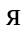
\includegraphics[width=1em]{ressources/l2.png}&s&e\\
            \hline
        \end{tabular}
    \end{center}
    \end{aretenir}
    \symbol{"0800}
\note{cyrillique: slave; Europe de l'est}
\end{frame}
\section{Encodage universel}
\subsection{Nouvelle norme}
\begin{frame}
    \frametitle{Encodage universel - nouvelle norme}
\begin{itemize}
    \item Norme ISO-10646
    \item Chaque caractère, signe ou idéogramme est associé à un numéro unique appelé \textbf{point de code}.
    \item Capacité maximale: 32 bits.
\end{itemize}
    
\note{Avec ISO 8859, il n’est pas possible d’encoder un texte qui contient des caractères de plusieurs tables.}
\end{frame}
\begin{frame}
    \frametitle{}

    \begin{itemize}
        \item $2^{32} = 4294967296$ caractères possibles
        \item exemple: lettre \textbf{é} point de code \textbf{U+00E9}
    \end{itemize}

\end{frame}
\subsection{Représentation en mémoire}
\begin{frame}
    \frametitle{Représentation en mémoire}

\begin{aretenir}[]
    Quatre octets (32 bits) pour chaque caractère est très coûteux en mémoire. La norme \textbf{Unicode} (et particulièrement \textbf{UTF-8 pour Universal Transformation Format}) définit plusieurs techniques pour économiser de l’espace.
\end{aretenir}

\end{frame}
\begin{frame}
    \frametitle{}

    \begin{itemize}
        \item Si le \emph{bit de poids fort} (le plus à gauche) est 0, il s'agit d'un caractère ASCII codé sur les 7 bits suivants.
        \item Sinon les premiers bits de poids fort de l'octet indiquent le nombre d'octets utilisés à l'aide de 1 et se terminant par 0.
        \end{itemize}

        \begin{center}
            \begin{tabular}{|c|c|}
            \hline 
            Suite d'octets (en binaire) & Bits codant \\ 
            \hline 
            0xxxxxxx & 7 bits \\ 
            \hline 
            110xxxxx 10xxxxxx & 11 bits \\ 
            \hline 
            1110xxxx 10xxxxxx 10xxxxxx & 16 bits \\ 
            \hline 
            11110xxx 10xxxxxx 10xxxxxx 10xxxxxx & 21 bits \\ 
            \hline 
            \end{tabular}
            \captionof{table}{Encodage UTF-8}
            \end{center}
\end{frame}
\begin{frame}
    \frametitle{}
    \begin{center}
        \begin{tabular}{|c|c|}
        \hline 
        Suite d'octets (en binaire) & Bits codant \\ 
        \hline 
        0xxxxxxx & 7 bits \\ 
        \hline 
        110xxxxx 10xxxxxx & 11 bits \\ 
        \hline 
        1110xxxx 10xxxxxx 10xxxxxx & 16 bits \\ 
        \hline 
        11110xxx 10xxxxxx 10xxxxxx 10xxxxxx & 21 bits \\ 
        \hline 
        \end{tabular}
        \captionof{table}{Encodage UTF-8}
        \end{center}
    \begin{aretenir}[Remarque]
    Tous les caractères ASCII sont encodés sur 1 octet.
    \end{aretenir}

\end{frame}
\begin{frame}
    \frametitle{}
    \begin{center}
        \begin{tabular}{|c|c|}
        \hline 
        Suite d'octets (en binaire) & Bits codant \\ 
        \hline 
        0xxxxxxx & 7 bits \\ 
        \hline 
        110xxxxx 10xxxxxx & 11 bits \\ 
        \hline 
        1110xxxx 10xxxxxx 10xxxxxx & 16 bits \\ 
        \hline 
        11110xxx 10xxxxxx 10xxxxxx 10xxxxxx & 21 bits \\ 
        \hline 
        \end{tabular}
        \captionof{table}{Encodage UTF-8}
        \end{center}
\begin{itemize}
    \item<1-> lettre \textbf{é} point de code \textbf{U+00E9}
    \item<2-> $00E9_{hex} = 11101001_{bin}$, il faut 8 bits pour encoder la lettre \textbf{é}
\end{itemize}

\end{frame}
\begin{frame}
    \frametitle{}
\begin{center}
    $00E9_{hex} = 11101001_{bin}$, il faut 8 bits pour encoder la lettre \textbf{é}
\end{center}
    \begin{center}
        \begin{tabular}{|*{2}{c|}}
            \hline
            110xxxxx&10xxxxxx\\
            \hline
110xxx\textbf{11}&10\textbf{101001}\\
\hline
        \end{tabular}
    \end{center}

\end{frame}
\begin{frame}
    \frametitle{}
\begin{center}
    $00E9_{hex} = 11101001_{bin}$, il faut 8 bits pour encoder la lettre \textbf{é}
\end{center}
    \begin{center}
        \begin{tabular}{|*{2}{c|}}
            \hline
            110xxxxx&10xxxxxx\\
            \hline
110000\textbf{11}&10\textbf{101001}\\
\hline
        \end{tabular}
    \end{center}
Pour encoder la lettre \textbf{é} la norme UTF-8 utilise 2 octets.
\end{frame}
\begin{frame}
    \frametitle{}

    \begin{aretenir}[Remarques]
        La norme UTF-8 est utilisée dans:
    \begin{itemize}
        \item plus de 95\% des sites web,
        \item de nombreux langages de programmation (Python).
    \end{itemize}
    \end{aretenir}
\note{c'est pour ça qu'on peut mettre accents dans nom de variable}
\end{frame}
\end{document}